\icode{E-MD-MU-L3-261115-003}
如图所示，系在墙上的轻绳通过轻质动滑轮连接滑块 \( P\)、\(Q \)，两滑块的质量均为 \( \SI{2}{kg} \)，与水平地面间的动摩擦因数均为 \( 0.5 \)。现对 \( P \) 施加水平向左的拉力 \( F = \SI{60}{N} \)，使 \( P \) 向左匀加速直线运动，绕过动滑轮的两段轻绳始终水平，不计轻绳与滑轮间的摩擦。重力加速度 \( g \) 取 \( \SI{10}{m/s^2} \)，下列说法正确的是\paren[]
	
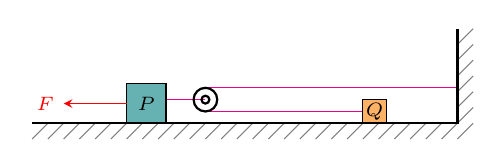
\begin{tikzpicture}[>=stealth,font=\scriptsize]
	\draw[magenta] (1,.15)--(3,.15) (1,.45)--(4.2,.45) (1,.3)--(.5,.3);
	\draw[thick] (1,.3) circle(.15) (1,.3) circle(.05);
	\draw[fill=orange!60] (3,0) rectangle(3.3,.3)node[pos=.5]{\(Q\)};
	\draw[fill=teal!60] (0,0) rectangle(.5,.5)node[midway]{\(P\)};
	\draw[red,->] (0,.25)--++(-.8,0)node[left]{\(F\)};
	\foreach \x in{-1.2,-1,...,4.2}
		\draw[gray] (\x,-.2)--++(.2,.2);
	\foreach \y in{0,.2,...,1}
		\draw[gray] (4.2,\y)--++(.2,.2);
	\draw[thick] (-1.2,0)--(4.2,0)--(4.2,1.2);
\end{tikzpicture}
\begin{choices}
	\item \( P \) 的加速度大小为 \(\SI{3}{m/s^2} \)
	\item \( Q \) 的加速度大小为 \(\SI{5}{m/s^2}\)
	\item 轻绳对 \( Q \) 的拉力大小为 \(\SI{22}{N} \)
	\item 轻绳对 \( Q \) 的拉力大小为 \(\SI{20}{N} \)
\end{choices}
\begin{answer}
	AC\qquad 提示：\(Q\)的加速度是\(P\)的两倍。
\end{answer}